\documentclass{article}

\usepackage{fullpage}
\usepackage{color}
\usepackage{amsmath}
\usepackage{url}
\usepackage{verbatim}
\usepackage{graphicx}
\usepackage{parskip}
\usepackage{amssymb}
\usepackage{nicefrac}
\usepackage{listings} % For displaying code
\usepackage{algorithm2e} % pseudo-code

% Answers
\def\ans#1{\par\gre{Answer: #1}}

% Colors
\definecolor{blu}{rgb}{0,0,1}
\def\blu#1{{\color{blu}#1}}
\definecolor{gre}{rgb}{0,.5,0}
\def\gre#1{{\color{gre}#1}}
\definecolor{red}{rgb}{1,0,0}
\def\red#1{{\color{red}#1}}
\def\norm#1{\|#1\|}

% Math
\def\R{\mathbb{R}}
\def\argmax{\mathop{\rm arg\,max}}
\def\argmin{\mathop{\rm arg\,min}}
\newcommand{\mat}[1]{\begin{bmatrix}#1\end{bmatrix}}
\newcommand{\alignStar}[1]{\begin{align*}#1\end{align*}}
\def\half{\frac 1 2}

% LaTeX
\newcommand{\fig}[2]{\includegraphics[width=#1\textwidth]{a4f/#2}}
\newcommand{\centerfig}[2]{\begin{center}\includegraphics[width=#1\textwidth]{a4f/#2}\end{center}}
\def\items#1{\begin{itemize}#1\end{itemize}}
\def\enum#1{\begin{enumerate}#1\end{enumerate}}


\begin{document}

\title{CPSC 340 Assignment 5 (due November 17 ATE)}
\author{}
\date{}
\maketitle
\vspace{-4em}

Name: Hang Yee Wong\\
CS ID: r9i0b

Name: Joanne Chen\\
CS ID: r0a9

\section{Multi-Class Logistic}

\subsection{Softmax Classification}

\enum{
\item The data has 2 features and 3 possible labels, and in multi-class classification we need a set of weights for each possible label.
\item $\hat{x} W =
\begin{bmatrix}
1 & 4 & 2
\end{bmatrix}$. So we select the label that corresponds to the entry with the highest value, and in this case it is label 2.
}

\subsection{Softmax Loss}

$$f_{W_{jc}}(W) = \sum_{i=1}^n \left[-I(y_i = c)x_{ij} + x_{ij}\exp(w_c^Tx_i)/\left(\sum_{c' = 1}^k \exp(w_{c'}^Tx_i)\right)\right]$$
$$\to f_{W_{jc}}(W) = \sum_{i=1}^n \left[-I(y_i = c)x_{ij} + x_{ij}p(c|W,x_i)\right]$$
$$\to f_{W_{jc}}(W) = \sum_{i=1}^n x_{ij}(p(c|W,x_i)-I(y_i = c))$$


\subsection{Softmax Classifier}

Code:
\begin{verbatim}
function softmaxObj(w,X,y,k)
    (n,d) = size(X)
    W = reshape(w,d,k)
    f = 0
    g = zeros(d,k)

    partial = function(j,c)
            total = 0
            for i in 1:n
                    term1 = y[i] == c ? 1 : 0
                    term2 = exp(W[:,c]'*X[i,:]) / sum(exp.(X[i,:]'*W))
                    total += X[i,j]*(term2-term1)
            end
            return total
    end

    for i in 1:n
            f += -W[:,y[i]]'*X[i,:] + log(sum(exp.(X[i,:]'*W)))
    end

    for j in 1:d
            for c in 1:k
                    g[j,c] = partial(j,c)
            end
    end

    return (f,reshape(g,d*k,1))
end

function softmaxClassifier(X,y)
    (n,d) = size(X)
    k = maximum(y)

    W = zeros(d,k)
    Wp = reshape(W,d*k,1)

    funObj(w) = softmaxObj(w,X,y,k)

    Wp = findMin(funObj,Wp,derivativeCheck=true,verbose=false)
    W = reshape(Wp,d,k);
    @show(W)

    predict(Xhat) = mapslices(indmax,Xhat*W,2)

    return LinearModel(predict,W)
end
\end{verbatim}

Using softmax, the new train error is 0.004 and the validation error is 0.026.

\subsection{Cost of Multinomial Logistic Regression}

Assuming that we have
\items{
\item $n$ training examples.
\item $d$ features.
\item $k$ classes.
\item $t$ testing examples.
\item $T$ iterations of gradient descent for training.
}
\enum{
\item Computing the derivative of the objective function with respect to one entry in $W$ takes $n(d + dk)$ time. We need to take the derivatives with respect to all entries in $W$ to get the gradient, so computing the gradient takes $dk(nd + ndk)$ time. Using gradient descent we compute the gradient $T$ times so the total cost is $T(knd^2 + nk^2d^2)$, which is in $O(Tnk^2d^2)$
\item To predict, we must compute $XW$, which takes $tdk$ time, and then we find the max of each training example, which takes $tk$, so the total is $tdk + tk$, which is in $O(tdk)$
}



\section{MAP Estimation}

In class, we considered MAP estimation in a regression model where we assumed that:
\items{
\item The likelihood $p(y_i | x_i, w)$ is a normal distribution with a mean of $w^Tx_i$ and a variance of $1$.
\item The prior for each variable $j$, $p(w_j)$, is a normal distribution with a mean of zero and a variance of $\lambda^{-1}$.
}
Under these assumptions, we showed computing the MAP estimate with $n$ training examples leads to the standard L2-regularized least squares objective function:
\[
f(w) = \frac{1}{2}\norm{Xw - y}^2 + \frac \lambda 2 \norm{w}^2.
\]
\blu{For each of the alternate assumptions below, write down the objective function that results} (from minimizing the negative log-posterior, and simplifying as much as possible):
\enum{
\item We use a Laplace likelihood with a mean of $w^Tx_i$ and a scale of $1$, and a normal prior with a variance of $\lambda^{-1}$ and a mean that is some ``guess'' $w^0$ of the optimal parameter vector,
\[
p(y_i | x_i, w) = \frac 1 2 \exp(-|w^Tx_i - y_i|), \quad p(w_j) \propto \exp\left(-\frac{\lambda(w_j -  w^0_j)^2}{2}\right)
\]
\item We use a normal  likelihood with a mean of $w^Tx_i$ but where each example $i$ has its own  positive variance $\sigma_i^2$, and we use a zero-mean Laplace prior for each variable with a scale parameter of $\lambda^{-1}$,
\[
p(y_i | x_i,w) = \frac{1}{\sqrt{2\sigma_i^2\pi}}\exp\left(-\frac{(w^Tx_i - y_i)^2}{2\sigma_i^2}\right), \quad p(w_j) = \frac{\lambda}{2}\exp(-\lambda|w_j|).
\]
The standard notation for this case is to use $\Sigma$ as a diagonal matrix with the $\sigma_i^2$ values along the diagonal.
\item We use a Poisson likelihood with a mean of $\exp(w^Tx_i)$,\footnote{This is one way to use regression to model \emph{counts}, like ``number of Facebook likes''.} and a zero-mean normal prior with a variance of $\sigma^2$,
\[
p(y_i | x_i, w) = \frac{\exp(y_iw^Tx_i)\exp(-\exp(w^Tx_i))}{y_i!}, \quad p(w_j) = \frac{1}{\sqrt{2\sigma_i^2\pi}}\exp\left(-\frac{(w_j - 0)^2}{2\sigma_i^2}\right).
\]
For this sub-question you don't need to put likelihood in matrix notation.
}


\enum{
\item $-\sum_{i=1}^n\log   \frac 1 2 \exp(-|w^Tx_i - y_i|)  -\sum_{i=1}^n\log \exp \frac{-\lambda(w_j -  w^0_j)^2}{2}$ \\
        $ =  \sum_{i=1}^n |w^Tx_i - y_i| +\sum_{i=1}^n  \frac{\lambda}{2}(w_j -  w^0_j)^2 + constant$\\
       $= \norm{Xw-y}_1 +  \frac{\lambda}{2} \norm{w_j -  w^0_j}^2 + constant$
\item  $-\sum_{i=1}^n\log  \frac{1}{\sqrt{2\sigma_i^2\pi}}\exp\left(-\frac{(w^Tx_i - y_i)^2}{2\sigma_i^2}\right) -\sum_{i=1}^n\log \frac{\lambda}{2}\exp(-\lambda|w_j|)  $\\
       $  =\sum_{i=1}^n( \frac{(w^Tx_i - y_i)^2}{2\sigma_i^2}+ constant) +  \sum_{i=1}^n (\lambda|w_j| +constant) $\\
       $ = \frac{1}{2}(Xw-y)^T \Sigma^{-1} (Xw-y) +\lambda|w|+ constant $
\item  $-\sum_{i=1}^n\log  \frac{\exp(y_iw^Tx_i)\exp(-\exp(w^Tx_i))}{y_i!} -\sum_{i=1}^n \log  \frac{1}{\sqrt{2\sigma_i^2\pi}}\exp\left(-\frac{(w_j - 0)^2}{2\sigma_i^2}\right)$\\
        $= -\sum_{i=1}^n (y_iw^Tx_i) + \sum_{i=1}^n \exp(w^Tx_i) +\frac{1}{2\sigma}\norm{w}^2+ constant$
}


\section{Principal Component Analysis (2016)}

\subsection{PCA by Hand}

Consider the following dataset, containing 5 examples with 2 features each:
\begin{center}
\begin{tabular}{cc}
$x_1$ & $x_2$\\
\hline
-2 & -1\\
-1 & 0\\
0 & 1\\
1 & 2\\
2 & 3\\
\end{tabular}
\end{center}
Recall that with PCA we usually assume that the PCs are normalized ($\norm{w} = 1$), we need to center the data before we apply PCA, and that the direction of the first PC is the one that minimizes the orthogonal distance to all data points.
\blu{
\enum{
\item What is the first principal component?
\item What is the (L2-norm) reconstruction error of the point (3,3)? (Show your work.)
\item What is the (L2-norm) reconstruction error of the point (3,4)? (Show your work.)
}
}

\enum{
\item The first principal component is $(\frac{1}{\sqrt2},\frac{1}{\sqrt2})$
\item $ z = (3-0)/ \sqrt2 +(3-1)/ \sqrt2 = 5/\sqrt2$ \\
        $ xhat = 5/\sqrt2 (\frac{1}{\sqrt2},\frac{1}{\sqrt2}) +(0,1) = (2.5,3.5)$\\
       $ reconstruction error = \sqrt{ (2.5-3)^2+(3-3.5)^2} = \frac{1}{\sqrt2} $
\item $ z = (3-0)/ \sqrt2 +(4-1)/ \sqrt2 = 6/\sqrt2$ \\
        $ xhat = 6/\sqrt2 (\frac{1}{\sqrt2},\frac{1}{\sqrt2}) +(0,1) = (3,4)$\\
       $ reconstruction error = \sqrt{ (3-3)^2+(4-4)^2} = 0 $
}


\subsection{Data Visualization}

The script \emph{example\_PCA} will load a dataset containing 50 examples, and measuring 85 binary traits of these animals. It then standardizes these features and gives two unsatisfying visualizations of it. First it shows a plot of the matrix entries, which has too much information and thus gives little insight into the relationships between the animals. Next it shows a scatterplot based on two random features and displays the name of 10 randomly-chosen animals. Because of the binary features even a scatterplot matrix shows us almost nothing about the data.

The function \emph{PCA}, which applies the classic PCA method (orthogonal bases via SVD) for a given $k$. Using this function, modify the demo so that the scatterplot uses the latent features $z_i$ from the PCA model. Make a scatterplot of the two columns in $Z$, and use the \emph{annotate} function to label a bunch of the points in the scatterplot.
\blu{
\enum{
\item  Hand in your modified demo and the scatterplot.
\item Which trait of the animals has the largest influence (absolute value) on the first principal component? (Make sure not to forget the ``+1'' when looking for the name of the trait in the \emph{dataTable}).
\item Which trait of the animals has the largest influence (absolute value) on the second principal component?
}
}

\begin{enumerate}
\item  Code: 
\begin{verbatim}
# Load data
dataTable = readcsv("animals.csv")
X = float(real(dataTable[2:end,2:end]))
(n,d) = size(X)



function FrobeniusNorm(X)
     X0 = X.^2
     X1 = sum(X0)
     return X1
end

function VarianceRemain(ZW,X)

    return 1- vecnorm(ZW-X).^2/vecnorm(X).^2
end

# Standardize columns
include("misc.jl")
(X,mu,sigma) = standardizeCols(X)


include("PCA.jl")
k =13
model = PCA(X,k)

Z = model.compress(X)
ZW=model.expand(Z)

print(VarianceRemain(ZW,X))

# Plot matrix as image
using PyPlot
figure(1)
clf()
imshow(X)

# Show scatterplot of 2 random features

figure(2)
clf()
plot(Z[:,1],Z[:,2],".")
for i in (1:n)
    annotate(dataTable[i+1,1],
    xy=[Z[i,1],Z[i,2]],
    xycoords="data")
end

\end{verbatim}


\begin{figure}[h!]
    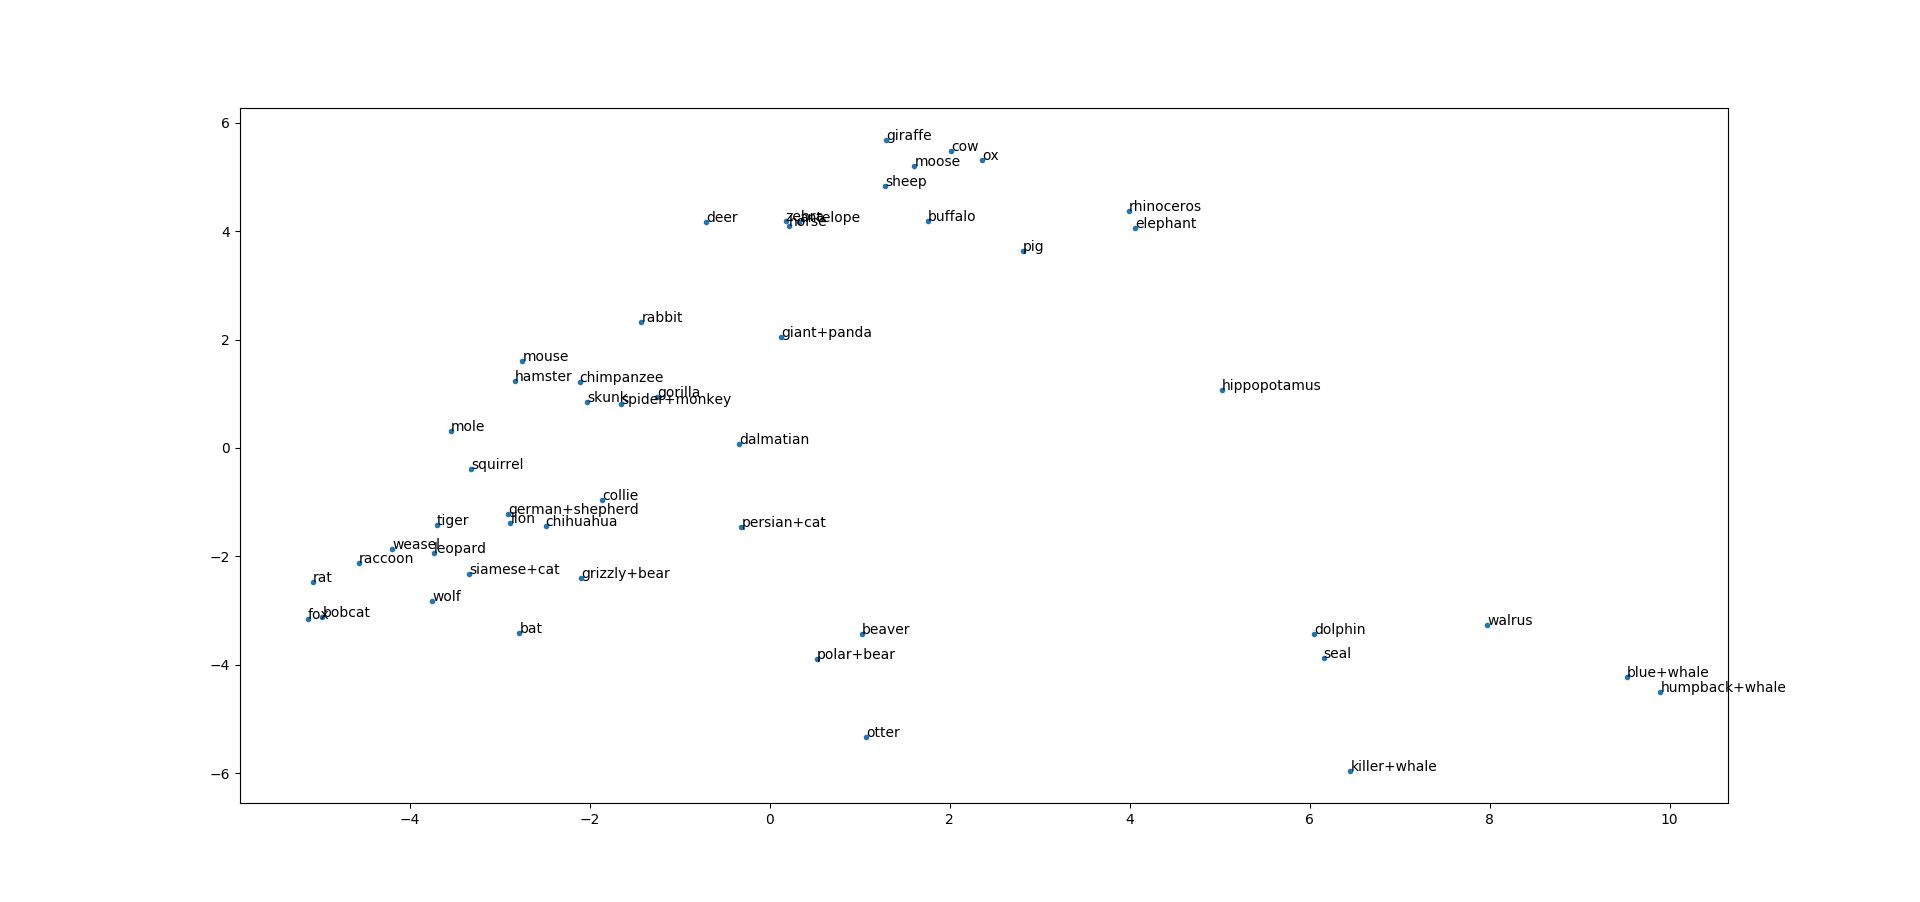
\includegraphics[width=50em,height=8.5cm]{q3_2_1_a.png}
\end{figure}
\item furry
\item grazer
\end{enumerate}


\subsection{Data Compression}

It is important to know how much of the information in our dataset is captured by the low-dimensional PCA representation.
In class we discussed the ``analysis" view that PCA maximizes the variance that is explained by the PCs, and the connection between the Frobenius norm and the variance of a centered data matrix $X$. Use this connection to answer the following:
\blu{\enum{
\item How much of the variance is explained by our two-dimensional representation from the previous question?
\item How many\ PCs are required to explain 50\% of the variance in the data?
\item How many\ PCs are required to explain 75\% of the variance in the data?
}}
Note: you can compute the Frobenius norm of a matrix using the function \emph{vecnorm}.

\enum{
\item 30.19\% 
\item K = 5
\item K = 14
}


\section{Very-Short Answer Questions}


\enum{
\item Stochastic gradient methods use the gradient computed from one data point at each step instead of the gradient from all data points, so it's much faster when $n$ is large.
\item No, the minimum exists in a 'ball', the radius of which is proportional to the step size, so ideally we would decrease the step size as we draw closer to the optimal region to ensure convergence.
\item Multi-label: each data point may be assigned multiple labels. Mult-class: there are more than 2 labels.
\item In MLE, we're maximizing the probability of $y$ given $X, w$, but in MAP, we're maximizing the probability of $w$, given $X, y$.
\item No. Linear regression with one feature finds the line that has the minimal sum of the $y$ distances from the data points, whereas PCA with 2 features finds the line with the minimal sum of the perpendicular distances from teh data points.
\item No, because there are usually multiple ways to write the same vector space. For example, $\begin{bmatrix}1 & 0\end{bmatrix}$, $\begin{bmatrix}0 & 1\end{bmatrix}$ form the same vector space as $\begin{bmatrix}2 & 0\end{bmatrix}$, $\begin{bmatrix}0 & 2\end{bmatrix}$
\item 1) Linear regression with L1-regularization. 2) TODO
\item Can we always use the normal equations to solve non-negative least squares problems? No? Because the minimizer computed from normal equations may be negative. TODO
}

\end{document}
